\section{Method}

Our central design is to use neural activity in place of an externally recorded action within a predictive world model. The mind model observes EEG only up to the current visual state and must encode the information needed to predict what happens next. We first formulate this prediction task and its two model components, then describe the Lateralization-Aware Transformer (LAT) and training objectives.

\begin{figure}[t]
\centering
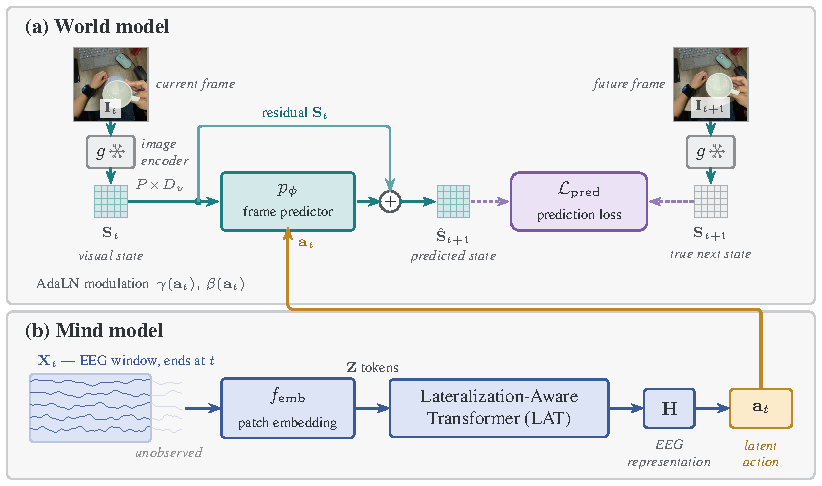
\includegraphics[width=\linewidth]{figures/mwm_overview.pdf}
\caption{\textbf{The Mind World Model.} \textbf{(a)} A frozen encoder $g$ maps the current
frame to patch features that a residual predictor advances; the same frozen $g$ builds
the target from the next frame. \textbf{(b)} The mind model encodes the EEG window, which
ends on the current frame; its LAT encoder is detailed in
Figure~\ref{fig:fliparch}. The EEG reaches the predictor only as AdaLN modulation, never as an
input token: it occupies the slot a recorded action would.}
\label{fig:mwm-framework}
\end{figure}

\subsection{Overview}

We propose the Mind World Model (\mwm{}) to jointly learn motor-related EEG representations and action-conditioned visual dynamics from synchronized EEG and egocentric video without action annotations. As illustrated in Figure~\ref{fig:mwm-framework}, \mwm{} consists of a world model and a mind model. Given an EEG segment $\mathbf{X}_t$ and a current frame $\mathbf{I}_t$, the mind model encodes the EEG into a latent action $\mathbf{a}_t$. The world model then predicts the representation of a future frame:
\begin{equation}
    \hat{\mathbf{S}}_{t+1}
    =
    p_{\phi}(\mathbf{S}_t,\mathbf{a}_t),
    \qquad
    \mathbf{S}_t=g(\mathbf{I}_t),
\end{equation}
where $g$ is a frozen image encoder and $p_{\phi}$ is a frame predictor. Future prediction both encourages the mind model to capture neural activity related to upcoming visual changes and trains the world model's dynamics and action interface.

In addition, we introduce LAT, an EEG encoder that explicitly models the lateralization of motor activity. It decomposes EEG features into bilateral and lateral components, which are respectively invariant and equivariant to swaps between homologous electrodes.

\subsection{Architecture}

A frozen visual encoder maps the current and future frames to patch tokens, and the world model advances the current token grid using a latent action encoded by LAT. Both models are trained jointly and retained separately. Motor decoders use the mind model; world-model evaluation freezes the predictor and maps IMU measurements to its action interface (Section~\ref{sec:world-action-probe}).

\subsubsection{World Model}

\paragraph{Image Encoder.}

Given a current frame $\mathbf{I}_t$ and its future frame $\mathbf{I}_{t+1}$, we use a frozen DINOv2 encoder $g$ to extract their spatial patch representations:
\begin{equation}
    \mathbf{S}_t=g(\mathbf{I}_t), \qquad
    \mathbf{S}_{t+1}=g(\mathbf{I}_{t+1}),
\end{equation}
where $\mathbf{S}_t,\mathbf{S}_{t+1}\in\mathbb{R}^{P\times D_v}$ and $P$ denotes the number of visual patches. We use patch-level features instead of a global feature because visual changes caused by hand and object movements are often spatially localized. The image encoder is kept frozen during training, providing a stable prediction target and preventing representation collapse.

\paragraph{Frame Predictor.}

The frame predictor models the transition from the current visual state to the future visual state, conditioned on EEG:
\begin{equation}
    \hat{\mathbf{S}}_{t+1}
    =
    p_{\phi}(\mathbf{S}_t,\mathbf{a}_t).
\end{equation}
We first project the EEG tokens into a compact conditioning vector $\mathbf{a}_t$. The current-frame tokens are then processed by a lightweight Transformer whose layers are modulated by $\mathbf{a}_t$ through adaptive layer normalization (AdaLN)~\citep{peebles2023scalable}:
\begin{equation}
    \operatorname{AdaLN}(\mathbf{h},\mathbf{a}_t)
    =
    \gamma(\mathbf{a}_t)\odot
    \operatorname{LN}(\mathbf{h})
    +
    \beta(\mathbf{a}_t).
\end{equation}
This design treats EEG as a latent action that controls the predicted visual transition. We further adopt residual prediction,
\begin{equation}
    \hat{\mathbf{S}}_{t+1}
    =
    \mathbf{S}_t+\Delta_{\phi}(\mathbf{S}_t,\mathbf{a}_t),
\end{equation}
such that the predictor focuses on dynamic changes instead of reconstructing the static scene.

To avoid temporal leakage, the EEG window ends at the current frame, while the prediction target is sampled from the subsequent time interval. Therefore, the target visual change is not already contained in the EEG observation window.

\subsubsection{Mind Model}

\paragraph{Transformers.}

Given an EEG segment $\mathbf{X}_t\in\mathbb{R}^{C\times T}$, we divide each channel into non-overlapping temporal patches. A channel-wise CNN embeds each patch by combining its temporal waveform and spectral representation, producing
\begin{equation}
    \mathbf{Z}_t
    =
    f_{\mathrm{emb}}(\mathbf{X}_t)
    \in\mathbb{R}^{C\times N\times D_e},
\end{equation}
where $C$ and $N$ denote the numbers of channels and temporal patches, respectively.

The EEG tokens are processed by a stack of criss-cross Transformer blocks. Each block separately performs temporal attention across patches and spatial attention across EEG channels. This factorization preserves the channel--time structure of EEG while reducing the cost of full attention. The resulting patch tokens are aggregated into the latent action $\mathbf{a}_t$ used by the frame predictor.

\begin{figure}[t]
\centering
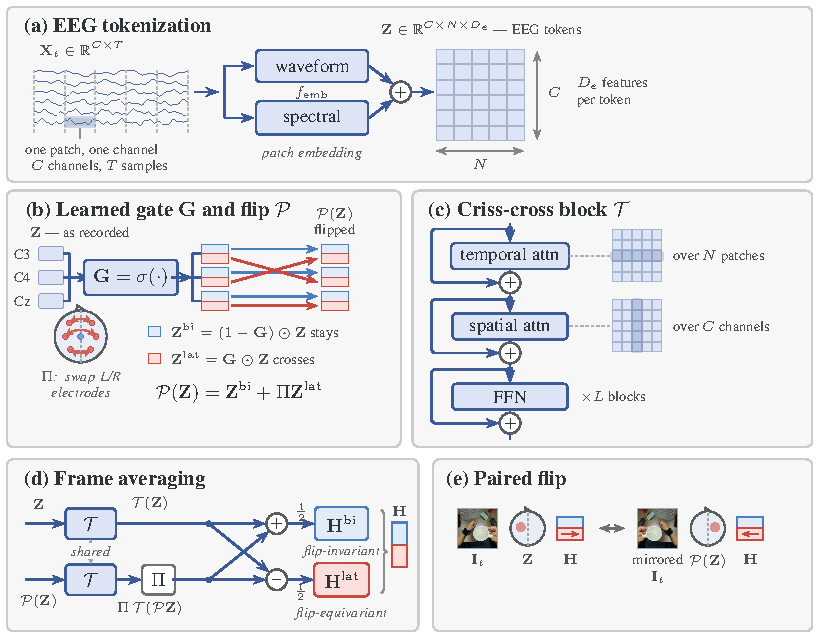
\includegraphics[width=\linewidth]{figures/mwm_flip.pdf}
\caption{\textbf{The Lateralization-Aware Transformer (LAT) for EEG encoding.} \textbf{(a)} Patch embedding, applied within each channel,
\textbf{(b)} the learned gate $\mathbf{G}$ and the electrode permutation $\Pi$, which act
on the embedded tokens before any Transformer block, \textbf{(c)} a criss-cross block,
\textbf{(d)} frame averaging into an invariant and an equivariant feature, and
\textbf{(e)} the paired EEG--video flip. Only the learned lateral component is exchanged
across hemispheres; the raw signal is never permuted.}
\label{fig:fliparch}
\end{figure}

\paragraph{Paired Flip Augmentation and LAT.}

EgoBrain contains substantially more right-hand than left-hand movements, reflecting the natural handedness distribution of its participants. Naively training on this dataset may therefore bias the learned representation toward right-hand activity. We alleviate this imbalance through paired EEG--video flip augmentation, realised by LAT in Figure~\ref{fig:fliparch}.

Let $\Pi$ denote the permutation that exchanges homologous electrodes across hemispheres, such as C3 and C4. Instead of directly swapping the raw EEG, we learn a gate $\mathbf{G}$ that decomposes each EEG token into bilateral and lateral components:
\begin{equation}
    \mathbf{Z}^{\mathrm{lat}}
    =
    \mathbf{G}\odot\mathbf{Z},
    \qquad
    \mathbf{Z}^{\mathrm{bi}}
    =
    (1-\mathbf{G})\odot\mathbf{Z}.
\end{equation}
We define the flip operation as
\begin{equation}
    \mathcal{P}(\mathbf{Z})
    =
    \mathbf{Z}^{\mathrm{bi}}
    +
    \Pi\mathbf{Z}^{\mathrm{lat}}.
\end{equation}
Thus, bilateral activity is preserved, while lateral activity is exchanged between the two hemispheres.

For a Transformer encoder $\mathcal{T}$, we apply frame averaging over the original and flipped representations:
\begin{align}
    \mathbf{H}^{\mathrm{bi}}
    &=
    \frac{1}{2}
    \left[
    \mathcal{T}(\mathbf{Z})
    +
    \mathcal{T}(\mathcal{P}(\mathbf{Z}))
    \right], \\
    \mathbf{H}^{\mathrm{lat}}
    &=
    \frac{1}{2}
    \left[
    \mathcal{T}(\mathbf{Z})
    -
    \Pi\mathcal{T}(\mathcal{P}(\mathbf{Z}))
    \right].
\end{align}
The final EEG representation concatenates the bilateral and lateral features:
\begin{equation}
    \mathbf{H}
    =
    \left[
    \mathbf{H}^{\mathrm{bi}};
    \mathbf{H}^{\mathrm{lat}}
    \right].
\end{equation}
By construction, the bilateral component is invariant to the flip, whereas the lateral component transforms equivariantly.

During training, we randomly flip each video horizontally and apply the corresponding operation $\mathcal{P}$ to its EEG representation. This augmentation balances left- and right-oriented movements while preserving their cross-modal correspondence.

\subsection{Training Objective}

\paragraph{Alignment Loss.}

We first align the global EEG representation $\mathbf{m}_i$ with the representation $\mathbf{v}_i$ of its synchronized frame. After projection and normalization, we compute their similarities as
\begin{equation}
    s_{ij}
    =
    \frac{
    \bar{\mathbf{m}}_i^\top\bar{\mathbf{v}}_j
    }{\tau},
\end{equation}
where $\tau$ is a temperature parameter. We use a symmetric InfoNCE objective:
\begin{equation}
    \mathcal{L}_{\mathrm{align}}
    =
    \frac{1}{2}
    \left[
    \operatorname{CE}(\mathbf{S},\mathbf{y})
    +
    \operatorname{CE}(\mathbf{S}^{\top},\mathbf{y})
    \right],
\end{equation}
where $\mathbf{y}_i=i$ denotes the matched EEG--frame pair.

The global image feature is nearly invariant to horizontal flipping and therefore provides limited supervision for lateralization. We additionally construct a flip-sensitive image representation by pooling the left and right spatial regions of the image-token grid. The representations of the original and mirrored frames are used as same-sample hard negatives, encouraging the lateral EEG features to distinguish the two orientations. We denote this objective as $\mathcal{L}_{\mathrm{flip}}$.

\paragraph{Prediction Loss.}

The primary world-model objective predicts the frozen representation of the future frame. We minimize the patch-level $\ell_1$ distance:
\begin{equation}
    \mathcal{L}_{\mathrm{pred}}
    =
    \frac{1}{BP}
    \sum_{i=1}^{B}
    \sum_{p=1}^{P}
    \left\|
    \hat{\mathbf{S}}_{i,t+1}^{p}
    -
    \mathbf{S}_{i,t+1}^{p}
    \right\|_1,
\end{equation}
Because the DINOv2 encoder $g$ is frozen, the visual target remains fixed throughout training. Minimizing this loss therefore requires the mind model to extract EEG information that explains the upcoming visual transition.

The overall objective is
\begin{equation}
    \mathcal{L}
    =
    \lambda_{\mathrm{align}}\mathcal{L}_{\mathrm{align}}
    +
    \lambda_{\mathrm{flip}}\mathcal{L}_{\mathrm{flip}}
    +
    \lambda_{\mathrm{pred}}\mathcal{L}_{\mathrm{pred}}.
\end{equation}
An auxiliary masked EEG reconstruction loss can be included to preserve low-level signal information, but future-state prediction remains the defining objective of \mwm{}.
